\documentclass[letterpaper]{article}
\usepackage{underscore}
\usepackage[left=3.0cm, right=3.0cm, top=3.0cm]{geometry}
\usepackage[utf8]{inputenc}
\usepackage{graphicx}
\usepackage{graphics}
\usepackage[spanish]{babel}
\usepackage{lipsum}
\usepackage{float}
\usepackage{subfigure}
\usepackage{color}
\usepackage{amssymb}

\title{Práctica 5, diseño del puente H}
\author{Carrasco Quiñones Karla Daniela y Reyna Gurrola Marcela}
\date{24 Octubre 2019}
\begin{document}
\maketitle
\begin{center}
    
\includegraphics[scale=1]{Imagenes/Logo.png}\\
    \vspace{1cm}
Sistemas Electrónicos de Interfaz\\
Ing.Mecatrónica
\end{center}\newpage


\section{Introdución}

 \begin{large}
En esta práctica se verá un poco sobre el funcionamiento de los puentes H, y se pretende mostrar como usarlos con la ayuda de un motor, lo que debe de hacer nuestro puente H es tener la capacidad de girar el motor y cambiar de dirección  del mismo al presionar dos botones; lo que hará este motor es: uno gira a la derecha por medio de un interruptor y al presionar el otro interruptor girará hacia la izquierda.
\end{large}




\section{Objetivo}
Saber cómo funcionan los puentes H para el control de motores.


\section{Materiales}
\begin{itemize}
    \item 2 Relevadores de 5V
    \item 4 Mosfets IRF640
    \item Resistencias varias
    \item Un motor DC de 5V
    \item Fuente de alimentación
    \item Protoboard
    \item Multímetro
\end{itemize}

\section{Procedimiento}
\begin{enumerate}
    \item Arma el esquema que se muestra en la figura 1. Ten en cuenta que el diodo led representa el motor, ya que el programa orcad no cuenta con este dispositivo.
    \item Conecta una fuente de voltaje de 5V a las "gates" y a los interruptores de los relevadores. Otra fuente del valor con el que funciona el motor alimentará al motor y los mosfets. 
    \item Para activar los relevadores puedes usar una fuente y un par de interruptores o utilizar el circuito hecho en la segunda práctica, donde se hizo uso un par de octocopladores y un arduino, el cual activa los relevadores.
\end{enumerate}

\newpage
\begin{figure}
        \centering
        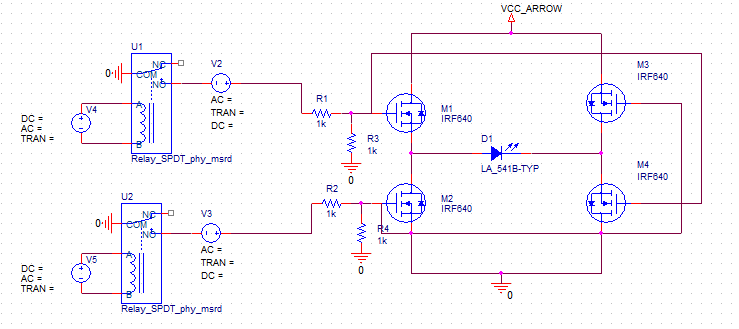
\includegraphics[scale=0.8]{Imagenes/Esquematico.png}
        \caption{Esquema}
        \label{fig:my_label}
    \end{figure}

\section{Resultados}
En esta práctica se utilizaron resistencias a la entrada de las gates, el valor se muestra en la ecuación 1.
\begin{center}
    \begin{equation}
        R = \frac{5V}{20mA} = 220\Omega
    \end{equation}
\end{center}
Y la resistencia que va a tierra se utilizó una de gran valor, ya que esta es la encargada de desactivar la gate.
Además cabe aclarar que el voltaje de entrada para el motor y los mosfets debe ser suficiente para alimentar el motor que se vaya a usar, en este caso es uno de 5V.
Se tomarón las medidas de voltaje de entrada de las "gates", asi como el voltaje de salida que alimenta al motor para comprobar que las conexiones eran correctas. Además de comprobar que la intensidad de la fuente que alimenta a las bobinas de los relevadores entregará la corriente necesaria.


\section{Conclusión}
Como se pudo observar con lo mencionado anteriormente los puentes H son de uso vital, ya que nos permiten manipular el giro del motor hacia ambos sentidos a voluntad, lo cual es muy conveniente al mover objetos en ambos sentidos. Además, se compredió en su totalidad el cómo funciona un mosfet; él como conduce mientras no se le aplique un pulso en la "gate", por esta razón es que se necesita una resistencia de gran valor a tierra, ya que permitirá descargar la compuerta de cualquier pulso y volver a permitir el paso de corriente en las terminales sobrantes.


\end{document}